\note{non inclus : 2 diagrammes de séquence du jeu de volley et 2 de WatchNDroid,
comme ca c'est joli, ca fait 2 pages par jeu.
Pour les remettre juste à décommenter}

\listoffigures

\clearpage
%% Pacman

\begin{figure}[h]
 \centering
 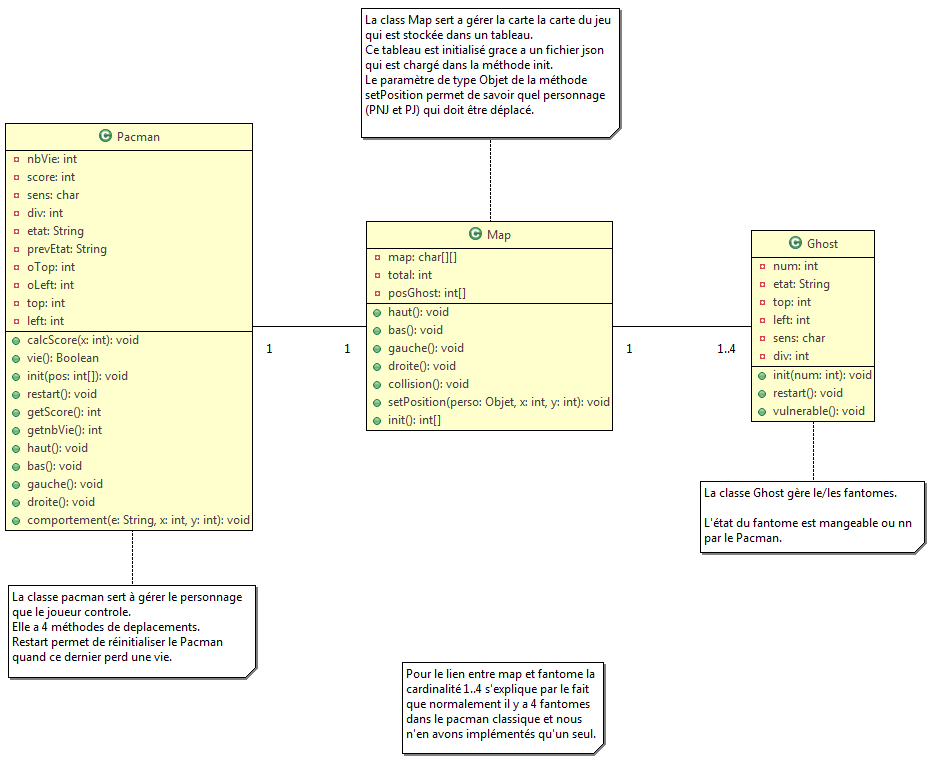
\includegraphics[width=\textwidth]{../umls/UML_images/Pacman/class} \hfill
 \caption{Diagramme de classe de Pacman}
\end{figure}

\begin{figure}[h]
 \centering
 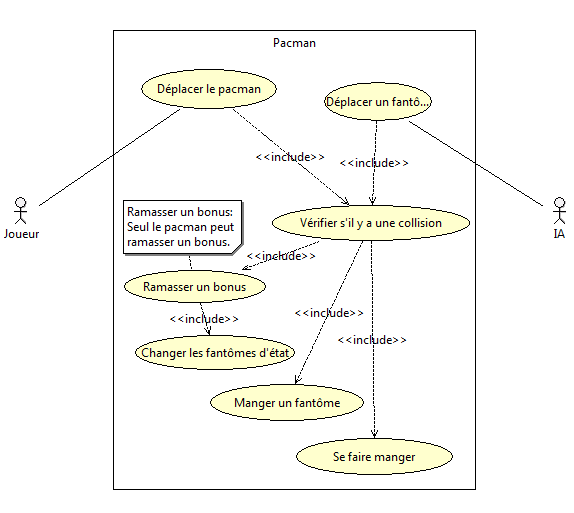
\includegraphics[width=10cm]{../umls/UML_images/Pacman/utilisation}
 \caption{Diagramme d'utilisation de Pacman}
\end{figure}

\begin{figure}[h]
 \centering
 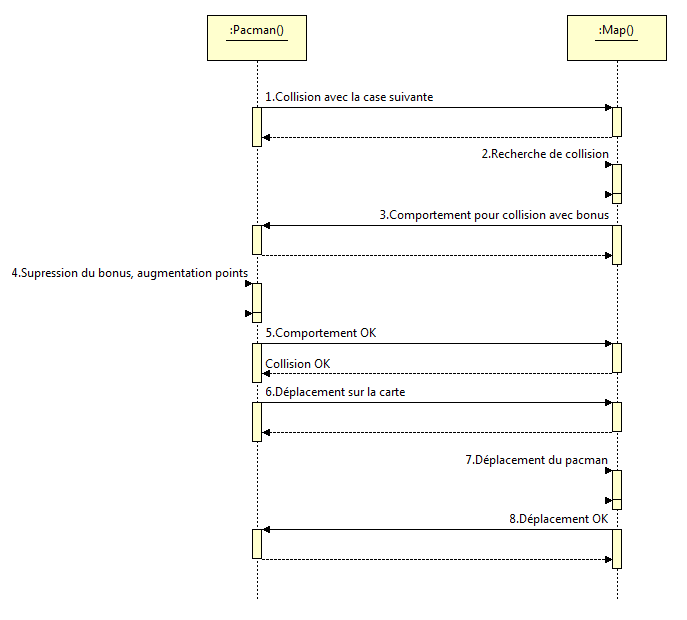
\includegraphics[width=9cm]{../umls/UML_images/Pacman/sequence} \hfill
 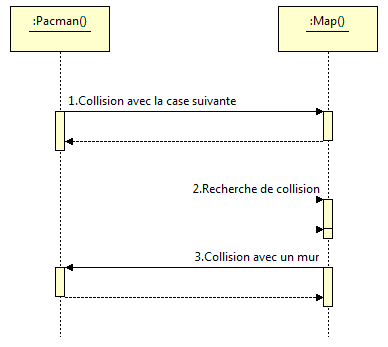
\includegraphics[width=6cm]{../umls/UML_images/Pacman/sequence2} \hfill
 \caption{Diagrammes de séquence de Pacman}
\end{figure}


\clearpage
%% 1942

\begin{figure}[h]
 \centering
 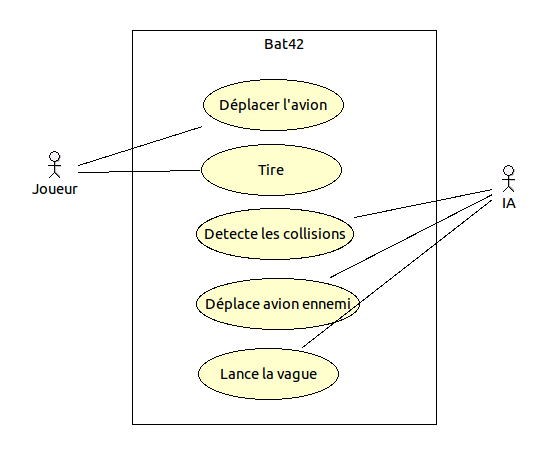
\includegraphics[height=6cm]{../umls/UML_images/Bat42/utilisation} \hfill
 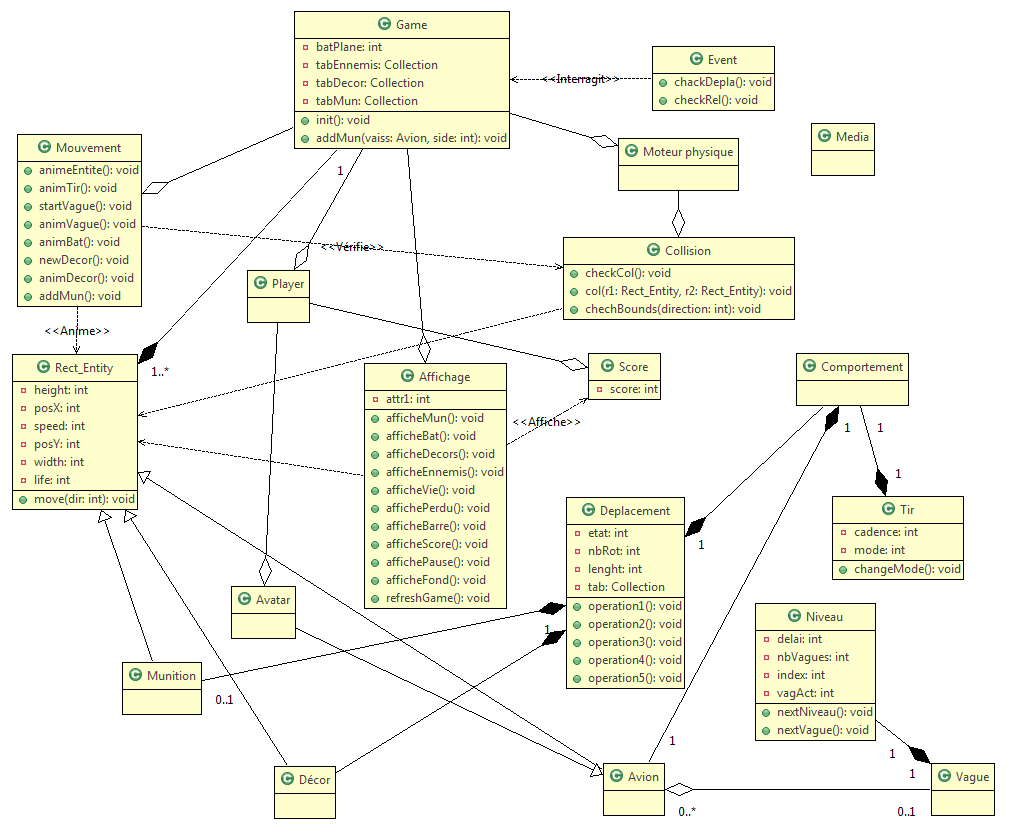
\includegraphics[height=13cm]{../umls/UML_images/Bat42/class} \hfill
 \caption{En haut, cas d'utilisation de 1942 ; en bas, son diagramme de classes}
\end{figure}

\begin{figure}[h]
 \centering
 \includegraphics[height=8cm]{../umls/UML_images/Bat42/sequence} \hfill
 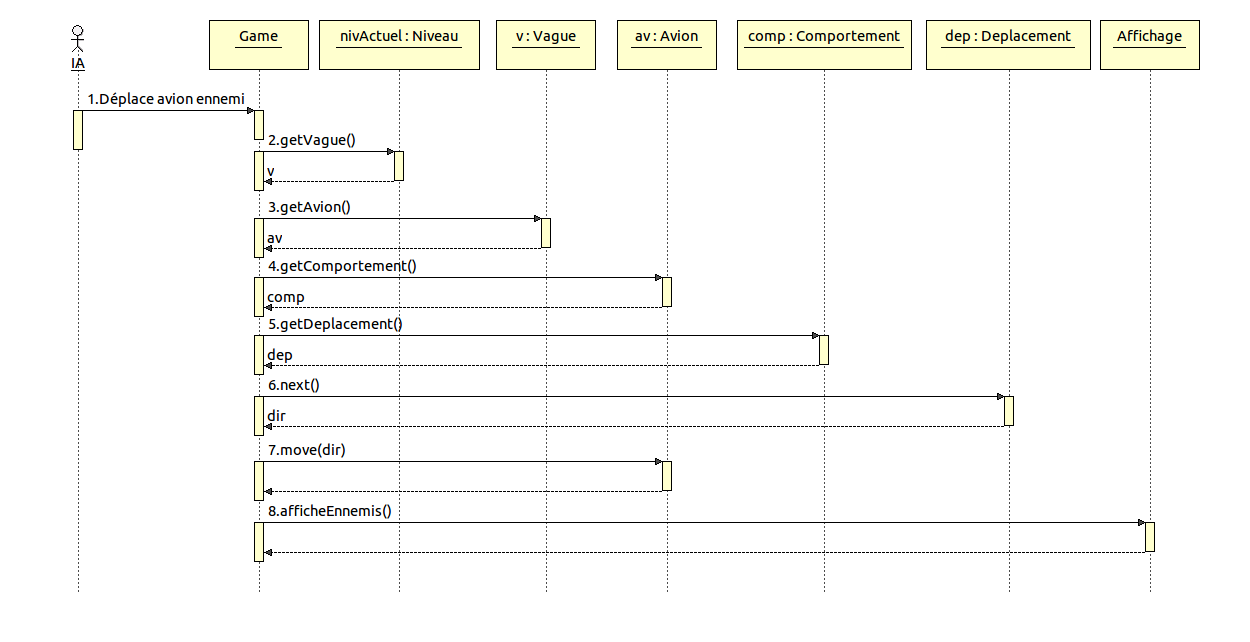
\includegraphics[width=\textwidth]{../umls/UML_images/Bat42/sequenceIA} \hfill
 \caption{Diagrammes de séquences de 1942}
\end{figure}

\clearpage
%% Volley

\begin{figure}[h]
 \centering
 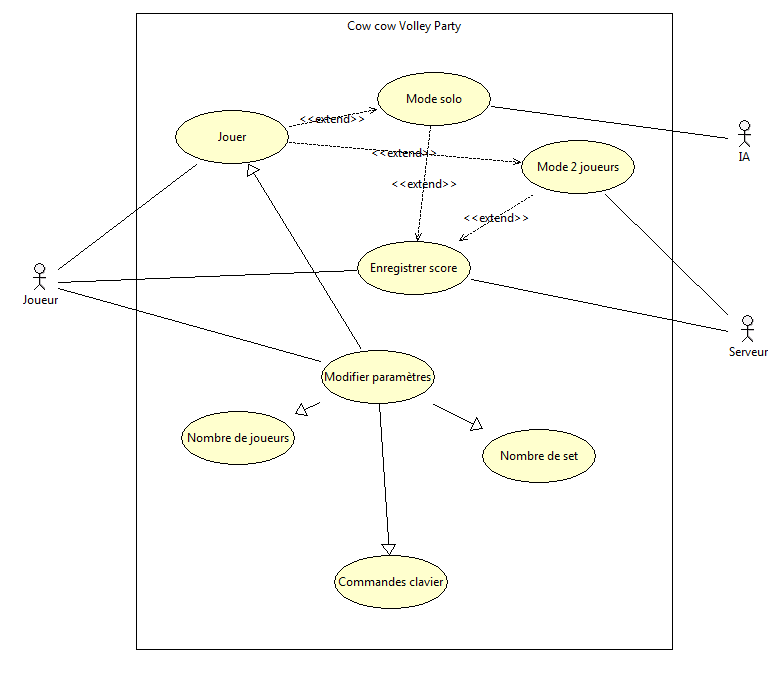
\includegraphics[height=8.5cm]{../umls/UML_images/Volley/utilisation} \hfill
 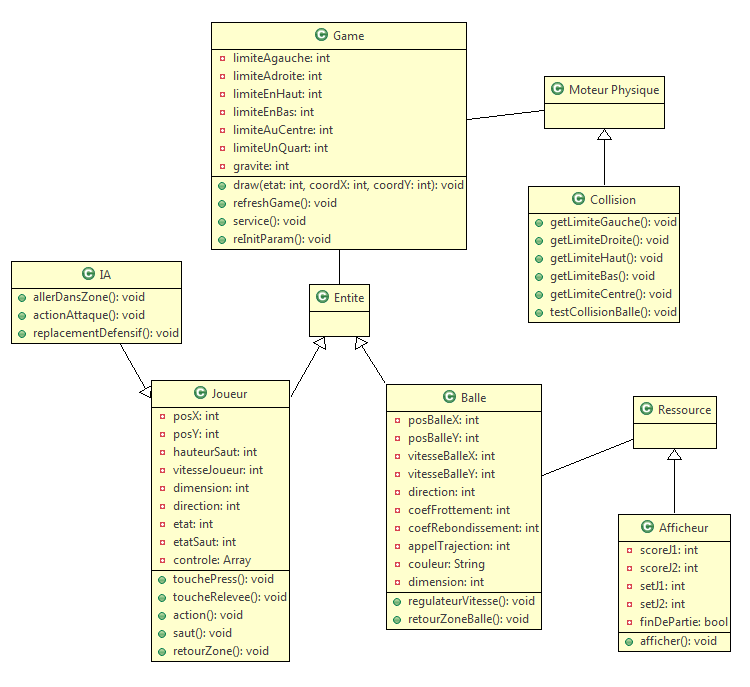
\includegraphics[height=11cm]{../umls/UML_images/Volley/class} \hfill
 \caption{En haut, cas d'utilisation du jeu de volley ; en bas, son diagramme de classes}
\end{figure}

\begin{figure}[h]
 \centering
 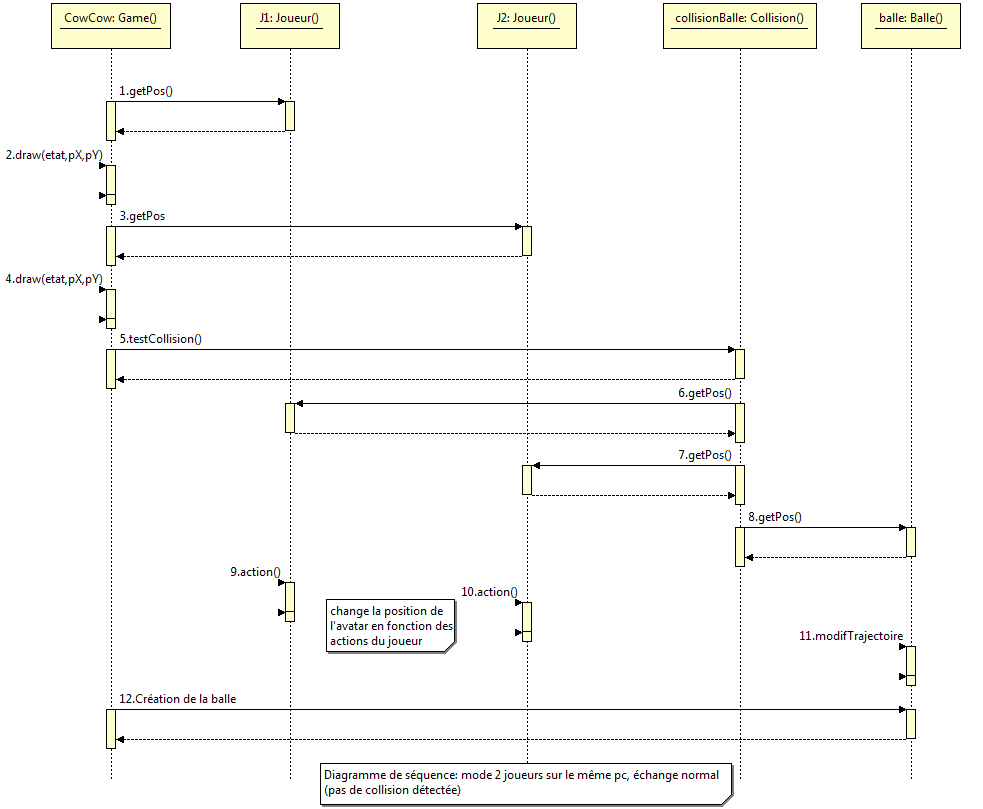
\includegraphics[height=9.5cm]{../umls/UML_images/Volley/sequence} \hfill
 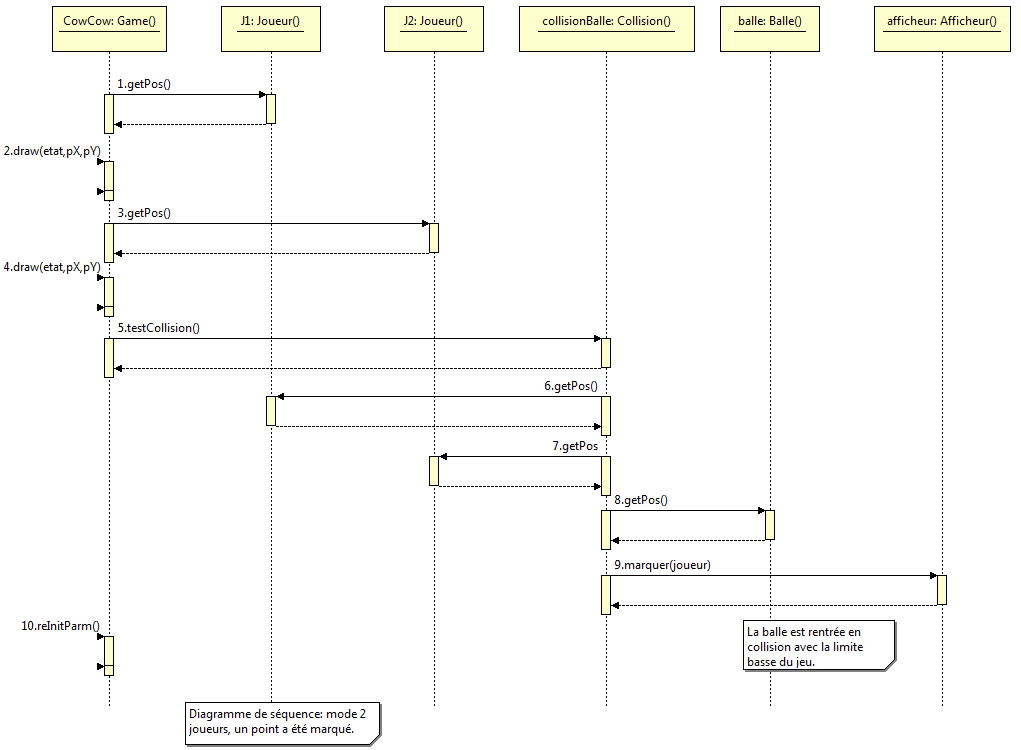
\includegraphics[height=10cm]{../umls/UML_images/Volley/sequence2} \hfill
 \caption{Diagrammes de séquences du jeu de volley}
\end{figure}

% \begin{figure}[h]
%  \centering
%  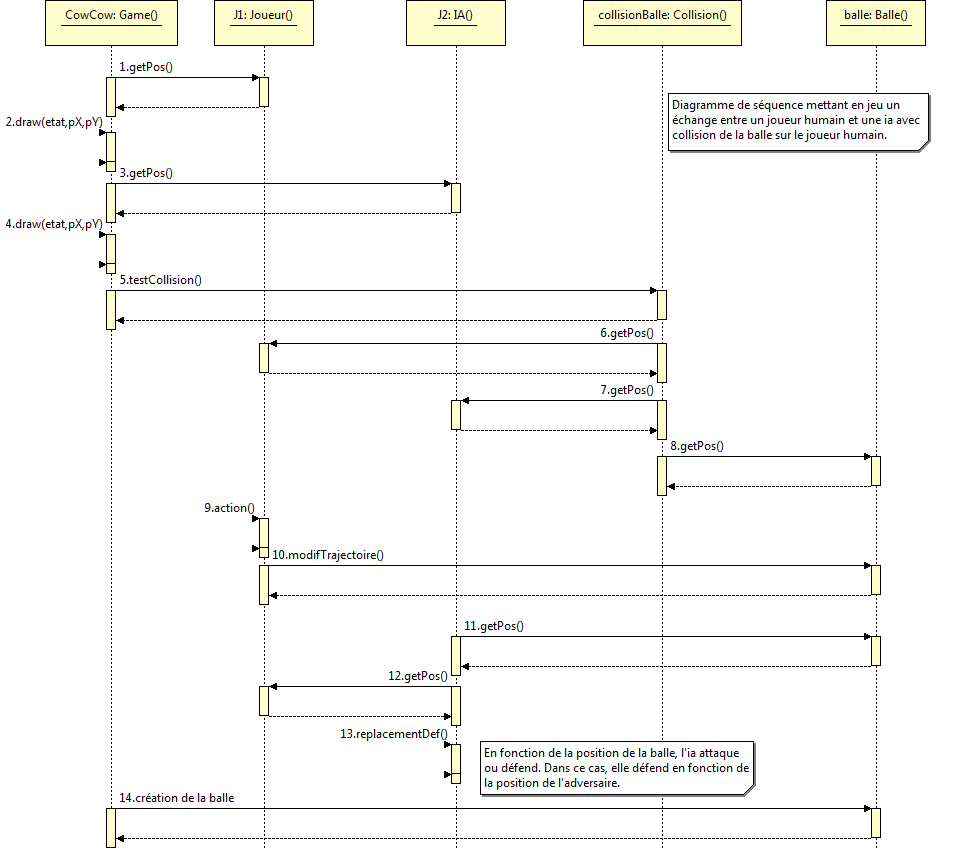
\includegraphics[height=9.5cm]{../umls/UML_images/Volley/sequence3} \hfill
%  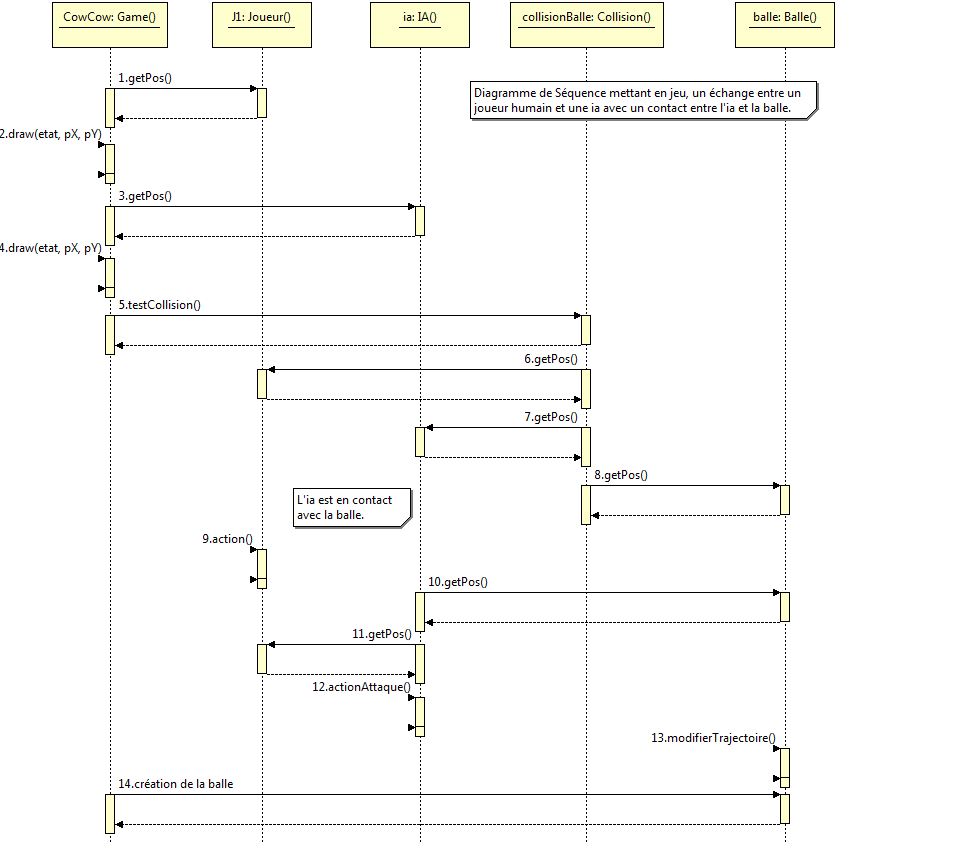
\includegraphics[height=10cm]{../umls/UML_images/Volley/sequence4} \hfill
%  \caption{Autres diagrammes de séquences du jeu de volley}
% \end{figure}

\clearpage
%% Course

\begin{figure}[h]
 \centering
 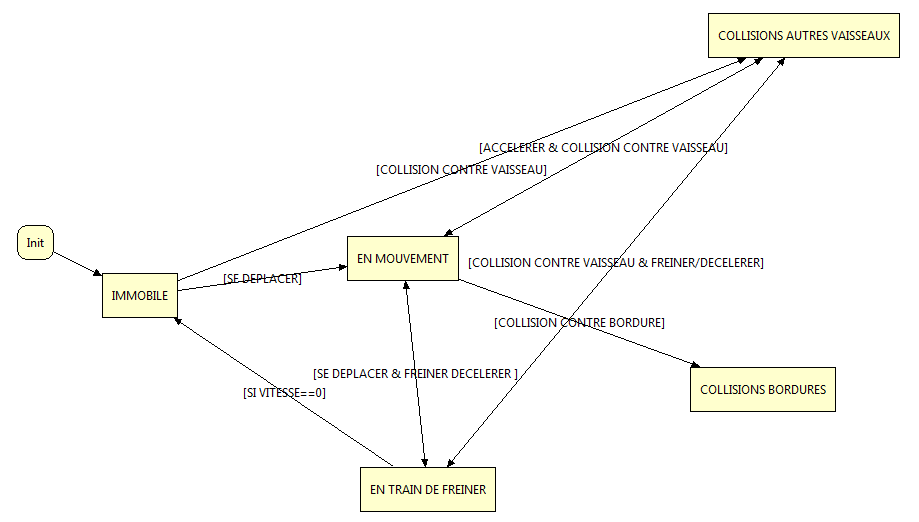
\includegraphics[width=\textwidth,height=9cm]{../umls/UML_images/course/activity} \hfill
 \includegraphics[width=\textwidth]{../umls/UML_images/course/class} \hfill
 \caption{En haut, diagramme d'activité du jeu de course ; en bas, son diagramme de classes}
\end{figure}

\begin{figure}[h]
 \centering
 \includegraphics[width=\textwidth]{../umls/UML_images/course/sequence} \hfill
 \caption{Diagramme de séquence du jeu de course}
\end{figure}

\clearpage
%% Mario

\begin{figure}[h]
 \centering
 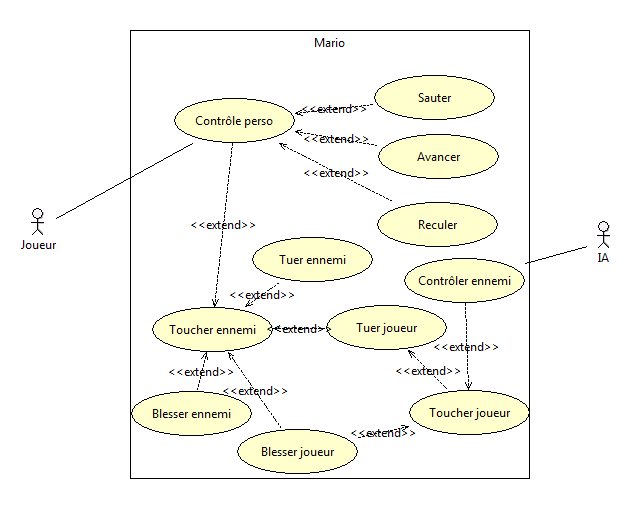
\includegraphics[width=\textwidth]{../umls/UML_images/Mario/Utilisation} \hfill
 \caption{Cas d'utilisation de Mario}
\end{figure}

\begin{figure}[h]
 \centering
 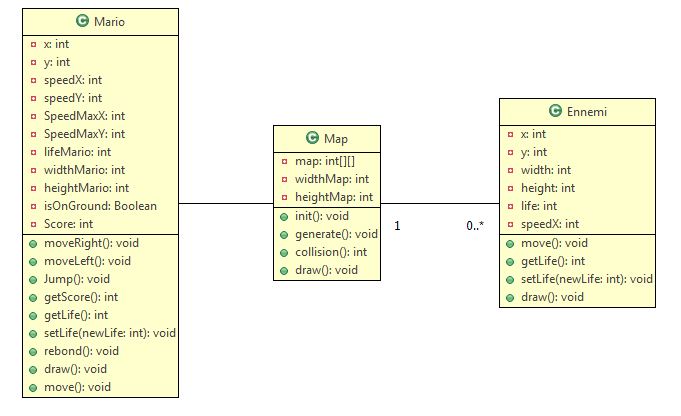
\includegraphics[height=9cm]{../umls/UML_images/Mario/Class} \hfill
 \caption{Diagramme de classes de Mario}
\end{figure}

\begin{figure}[h]
 \centering
 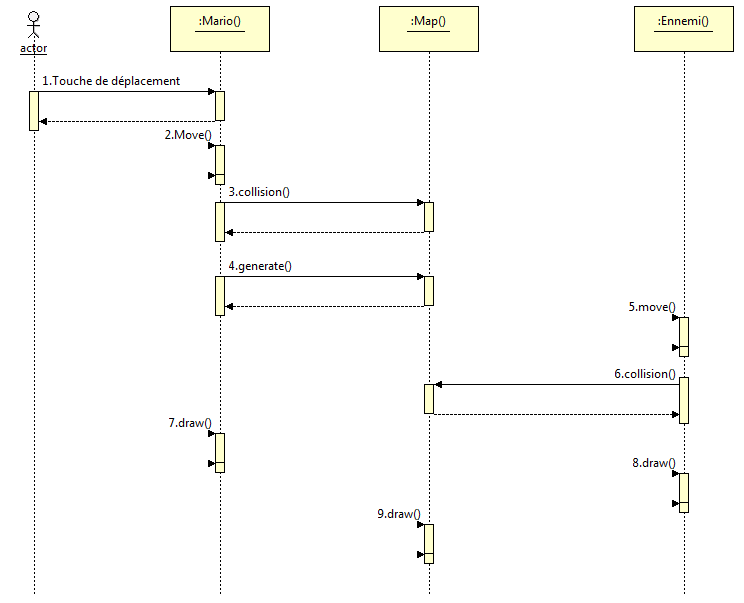
\includegraphics[height=11.5cm]{../umls/UML_images/Mario/Sequence} \hfill
 \caption{Diagramme de séquence de Mario}
\end{figure}


\clearpage
%% WatchNDroid

\begin{figure}[h]
 \centering
 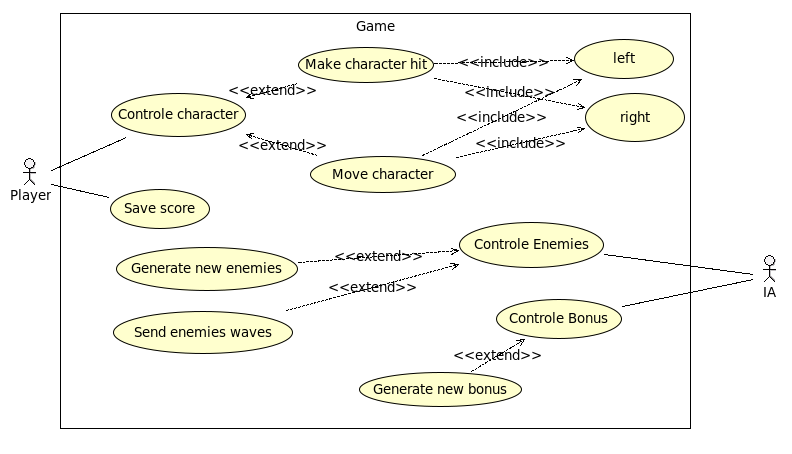
\includegraphics[height=8.5cm]{../umls/UML_images/WatchNDroid/utilisation} \hfill
 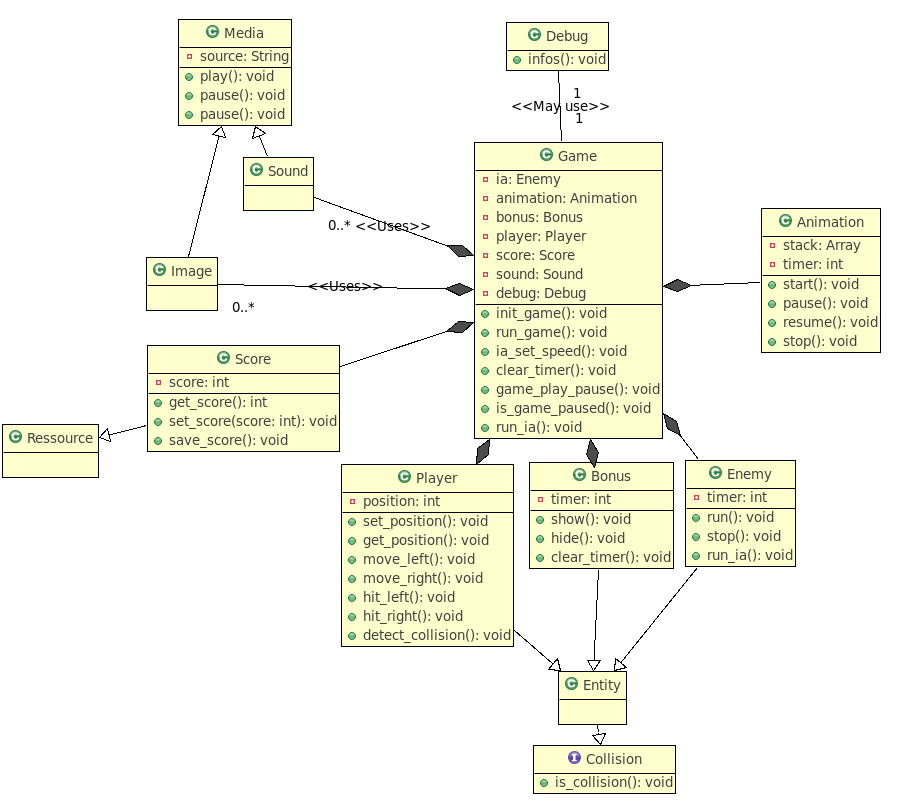
\includegraphics[height=11cm]{../umls/UML_images/WatchNDroid/class} \hfill
 \caption{En haut, cas d'utilisation du jeu Watch'N'Droid; en bas, son diagramme de classes}
\end{figure}

\begin{figure}[h]
 \centering
 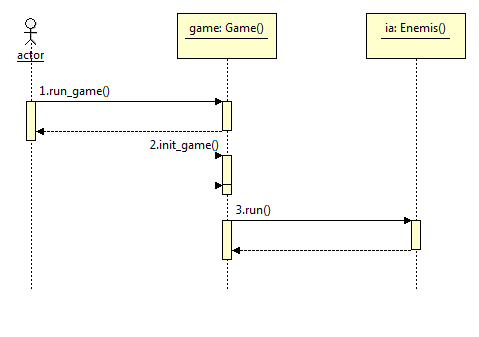
\includegraphics[height=9.5cm]{../umls/UML_images/WatchNDroid/sequence} \hfill
 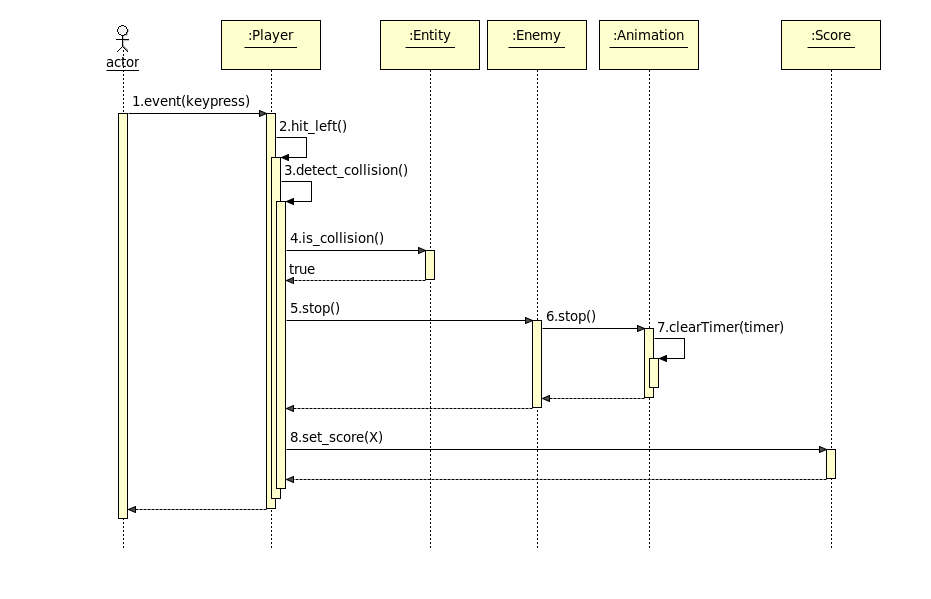
\includegraphics[height=10cm]{../umls/UML_images/WatchNDroid/sequence2} \hfill
 \caption{Diagrammes de séquences du jeu Watch'N'Droid}
\end{figure}

% \begin{figure}[h]
%  \centering
%  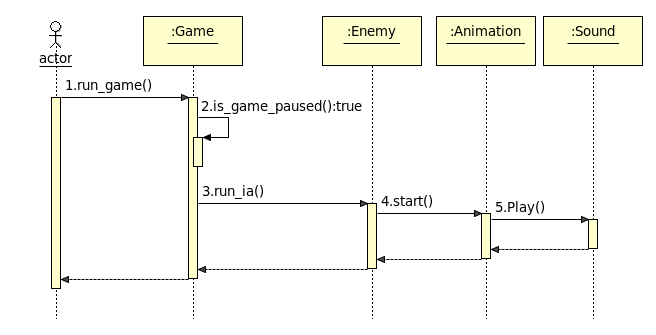
\includegraphics[height=8cm]{../umls/UML_images/WatchNDroid/sequence3} \hfill
%  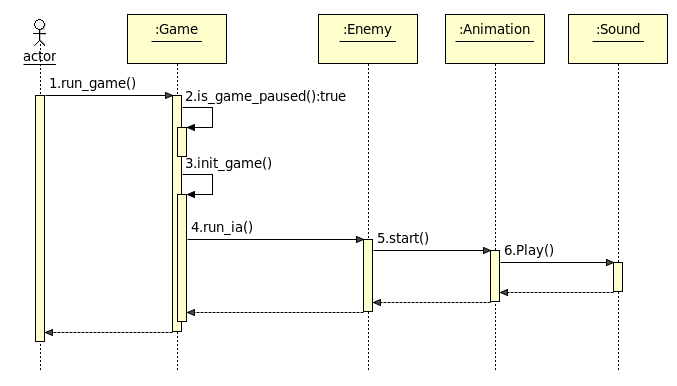
\includegraphics[height=8cm]{../umls/UML_images/WatchNDroid/sequence4} \hfill
%  \caption{Autres diagrammes de séquences du jeu Watch'N'Droid}
% \end{figure}

\clearpage
%% Billard

\begin{figure}[h]
 \centering
 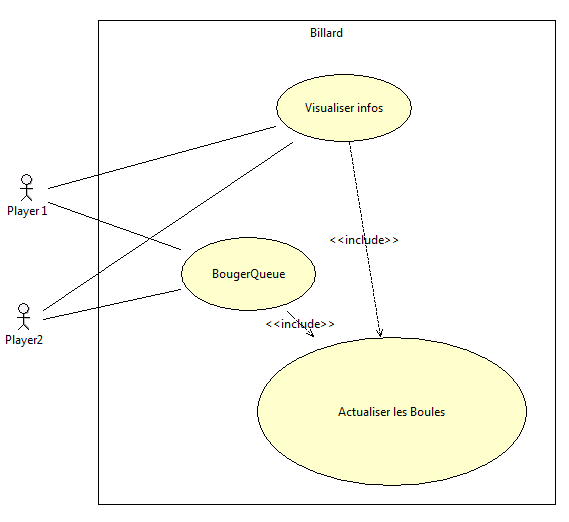
\includegraphics[height=7cm]{../umls/UML_images/Billard/utilisation} \hfill
 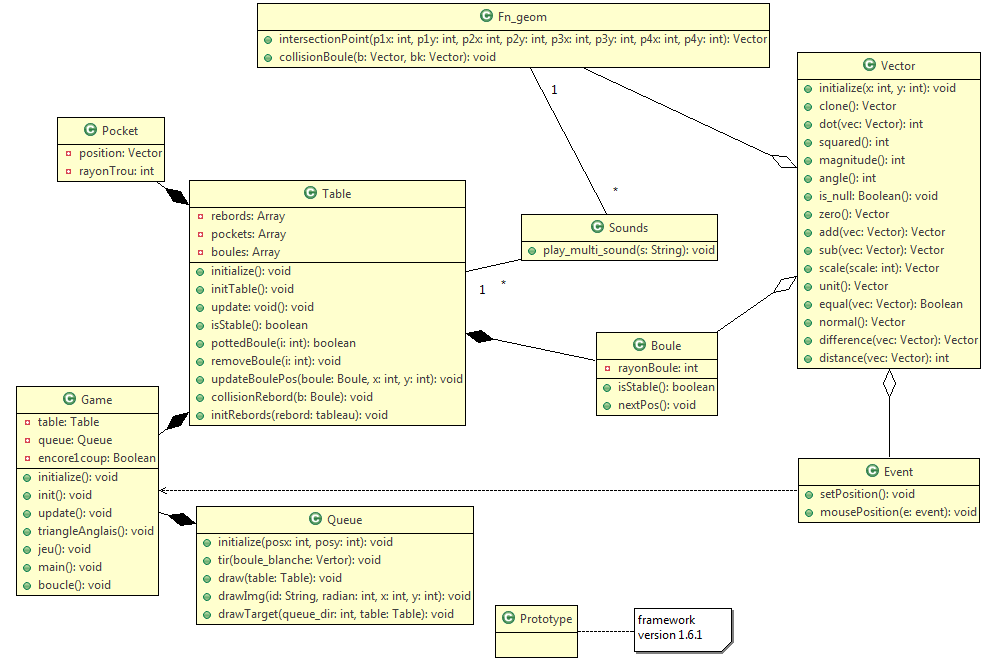
\includegraphics[width=\textwidth,height=12cm]{../umls/UML_images/Billard/class} \hfill
 \caption{En haut, les cas d'utilisation du billard ; en bas, son diagramme de classes}
\end{figure}

\begin{figure}[h]
 \centering
 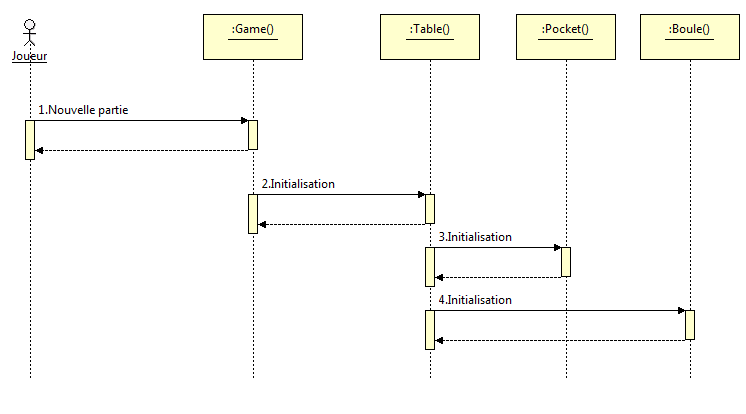
\includegraphics[height=6.5cm]{../umls/UML_images/Billard/sequence1} \hfill
 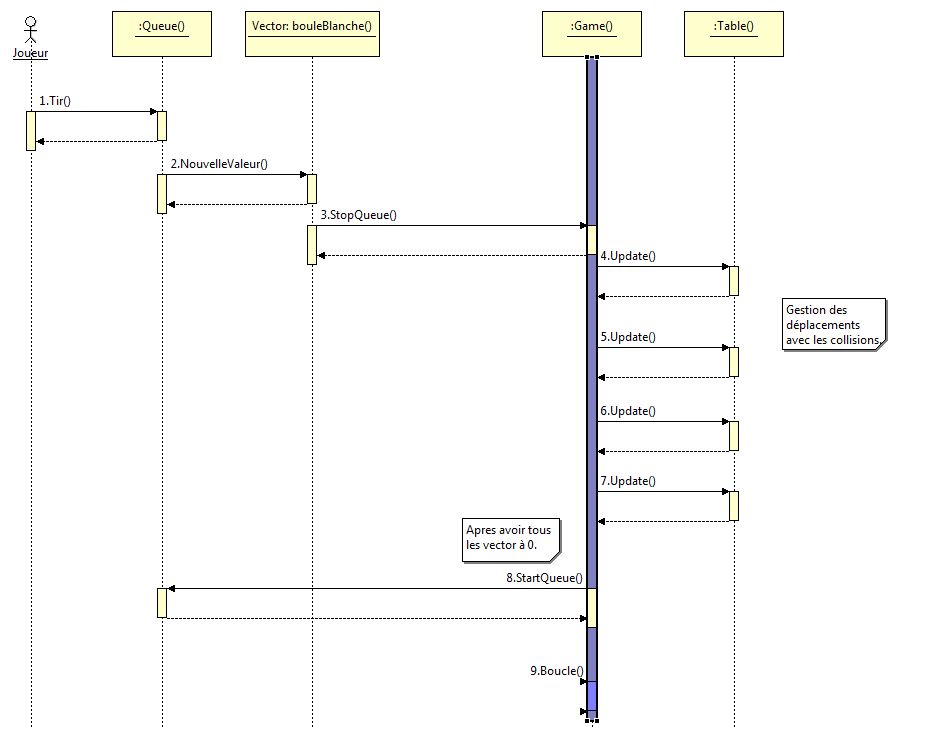
\includegraphics[height=11cm]{../umls/UML_images/Billard/sequence2} \hfill
 \caption{Diagrammes de séquence du billard}
\end{figure}

\clearpage
%% Commissariat

\begin{figure}[h]
 \centering
 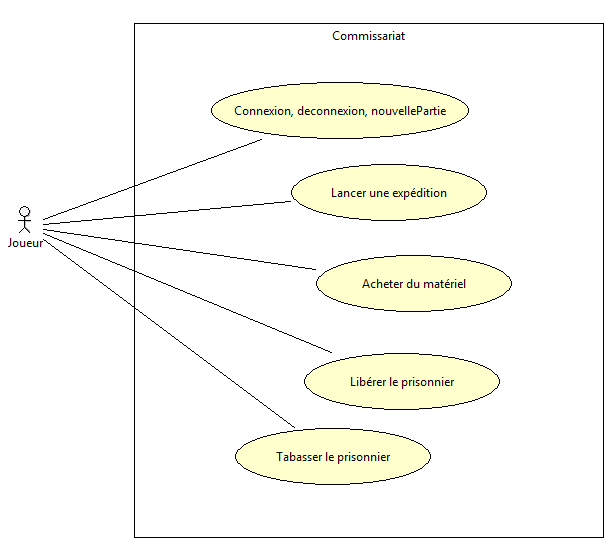
\includegraphics[width=\textwidth]{../umls/UML_images/Commissariat/utilisation} \hfill
 \caption{Cas d'utilisation du jeu de gestion}
\end{figure}

\begin{figure}[h]
 \centering
 \includegraphics[width=\textwidth]{../umls/UML_images/Commissariat/class} \hfill
 \caption{Diagramme de classes du jeu de gestion}
\end{figure}